\section{Introduzione}
L'equazione di diffusione in un corpo bidimensionale \`e
\[
	u_t= D(u_{xx}+ u_{yy} +f)
\]
mentre in un corpo a tre dimensioni (solido) \`e
\[
	u_t=D\left( u_{xx}+u_{yy} +u_{zz} \right) +f
\]
L'operatore 
\[
	\Delta= \partial_{x_1x_1}+ \ldots + \partial_{x_n x_n}
\]
in ogni dimensione $n$ \`e detto \textit{Laplaciano}. Con questa notazione
l'equazione di diffusione si scrive 
\[
	u_t= D\Delta u +f
\]
Nel caso di sorgenti $f$ non dipendenti dal tempo, \`e ragionevole cercare 
soluzioni stazionarie, cio\`e anch'esse indipendenti da $t$.
Si giunge cos\`i all'\textit{equazione di Poisson}
\[
	\Delta u= -f/D
\]
Nel caso omogeneo $f=0$, l'equazione
\[
	\Delta u=0
\]
si dice \textit{equazione di Laplace} e le soluzioni si dicono 
\textit{funzioni armoniche}.\\
Anche le soluzioni stazionarie dell'equazione
\[
	u_{tt}c^2 \Delta u
\]
sono funzioni armoniche. In dimensione di spazio $n=2$, questa equazione
descrive lo spostamento di una membrana elastica dalla posizione di riposo.
Una posizione stazionaria (equilibrio) \`e quindi descritta da una funzione
armonica.
Se $F=(f_1,f_2, f_3)=f_1= f_1 \uvi + f_2 \uvj + f_3 \uvk$ \`e un campo
vettoriale nello spazio, la divergenza di $F$ \`e lo scalare
\[
	div F= \partial_x f_1 + \partial_y f_2 + \partial_z f_3
\]
Se esiste una funzione scalare $u$ tale che
\[
	\nabla u= F
\]
(potenziale), allora
\[
	div F= div \nabla u = div \left( u_x \uvi +u_y \uvj + u_x \uvk \right)
	=\Delta u
\]
L'equazione di Laplace/Poisson \`e quindi fondamentale nello studio dei campi conservativi. Se $E$ \`e un campo elettrostatico in una regione $\Omega$
di spazio, allora si ha
\[
	div E= \frac{4 \pi \rho}{\varepsilon}
\]
con $\rho$ densit\`a di carica ed $\varepsilon$ costante dielettrica. Se
\[
	\Delta u= -E
\]
il potenziale soddisfa l'equazione di Poisson
\[
	\Delta u= - \frac{4 \pi \rho}{\varepsilon}
\]
Nel caso $\rho=0$, cariche fuori di $\Omega$, la funzione $u$ \`e armonica.
In dimensione $n=2$, le funzioni armoniche intervengono anche nello studio
di funzioni di variabile complessa.
Se $f= u+iv$ \`e derivabile in senso complesso, vale l'equazione di 
Cauchy- Riemann
\[
	\frac{\partial f}{\partial x}= \frac{1}{i} \frac{\partial f}
	{\partial y}
\]
che si scrive anche 
\[
	\left\{ 
	\begin{array}{l}
		u_x=v_y \\
		v_x=- u_y
	\end{array}
	\right.
\]
Dunque
\[
	\Delta u= u_{xx}+ u_{yy}= v_{yx}-v_{xy}=0
\]
\[
	\Delta v= v_{xx}+ v_{yy}= -u_{yx} +u_{xy}=0
\]
La parte reale $u$ e l parte immaginaria $v$ di $f$ sono funzioni
armoniche.
Viceversa, se $u$ \`e una funzione armonica, \`e possibile risolvere le
equazioni di Cauchy-Riemann rispetto a $v$ in ogni parte semplicemente connessa
del dominio in modo che 
\[
	f= u+ iv
\]
sia una funzione derivabile in senso complesso.
Tale funzione \`e in realt\`a derivabile infinite volte perch\'e si pu\`o
espandere localmente in serie di potenze. Ne segue che $u$ (e $v$) \`e
derivabile infinite volte in $dx$, $dy$.
Abbiamo cos\`i che una funzione armonica nel piano \`e derivabile infinite
cio\`e di classe $C^{\infty}$.
\section{Formule di Gauss-Green ed applicazioni al Laplaciano}
Se $\gamma$ \`e una curva chiusa nel piano, orientata in senso antiorario,
regolare (a tratti) con parametrizzazione
\[
	x= x(t), \;\;\; y=y(t), \;\;\; a\leq t \leq b
\]
Il versore tangente a $\gamma$
\[
	{\bf T}= \frac{1}{\sqrt{(x')^2+ (y')^2}}(x', y')
	=\frac{x'}{\sqrt{(x')^2+ (y')^2}}\uvi
	+\frac{y'}{\sqrt{(x')^2+ (y')^2}}\uvj
\]
Ora, per ottenere il versore normale ${\bf N}$, bisogna calcolare il versore
ortogonale a ${\bf T}$; ci\`o \`e ottenuto con
\[
	{\bf N}= \frac{1}{\sqrt{(x')^2+ (y')^2}}(y', -x')
	=\frac{y'}{\sqrt{(x')^2+ (y')^2}}\uvi
	-\frac{x'}{\sqrt{(x')^2+ (y')^2}}\uvj
\]
che rappresenta la normale esterna a $\gamma$; la normale interna \`e invece
\[
	{\bf N}= \frac{1}{\sqrt{(x')^2+ (y')^2}}(-y', x')
	=-\frac{y'}{\sqrt{(x')^2+ (y')^2}}\uvi
	+\frac{x'}{\sqrt{(x')^2+ (y')^2}}\uvj
\]
Dato un campo vettoriale $F= f_1 \uvi + f_2 \uvj$, gli integrali curvilinei
\[
	\int_ {\gamma} F \cdot {\bf T} ds= 
	\int_a^b \left[ f_1 (x(t), y(t))x'(t)+
	f_2 (x(t), y(t))y'(t)
	\right] dt
\]
\[
	\int_ {\gamma} F \cdot {\bf N} ds= 
	\int_a^b \left[ f_1 (x(t), y(t))y'(t)
	- f_2 (x(t), y(t))x'(t)
	\right] dt
\]
rappresentano, rispettivamente, il lavoro di $F$ su $\gamma$ ed il flusso
uscente di $F$ da $\Omega$. Si \`e fatto uso dello spostamento infinitesimo
\[
	ds= \sqrt{(x')^2+(y')^2}
\]

Le formule di Gauss-Green collegano gli integrali curvilinei su $\gamma$
ad integrali in $dx dy$ su $\Omega$:
\[
	\int_{\Omega}\partial_x f(x,y)dx dy= \int_{\gamma} f \uvj \cdot {\bf T} ds
\]
\[
	\int_{\Omega}\partial_y f(x,y)dx dy= - \int_{\gamma} f \uvi \cdot {\bf T} ds
\]
Tali formule sono di facile dimostrazione su domini normali. Ad esempio
preso $\Omega$ come in fig. \ref{nor_dom}
\begin{figure}[H]
	\centering
	\includegraphics[width=0.8\textwidth]{nor_dom.pdf}
	\caption{Dominio normale per la dimostrazione delle formule di Green}
	\label{nor_dom}
\end{figure}
\noindent
si ha
\[
	\int_{\Omega} \partial_y f (x,y) dx dy=
	\int_a^b \int_{\alpha(x)}^{\beta(x)}
	\partial_y f (x,y) dx dy=
	\int_a^b \left[
		f(x,y)
	\right]_{y=\alpha(x)}^{y=\beta(x)}dx
\]
\[
	= \int_a^b \left[
	f(x,\beta (x)) - f(x, \alpha(x))
	\right] dx
\]
Per il tratto di frontiera
\[
	\left\{ 
	\begin{array}{ll}
		x=x & x \in [a,b] \\
		y= \alpha(x)
	\end{array}
	\right.
\]
si ha
\[
	{\bf T}= \frac{1}{\sqrt{1+ (\alpha ' )^2}}(1,\alpha ')
\]
\[
	ds= \sqrt{1+ (\alpha ' )^2} dx
\]
\[
	{\bf T} \cdot \uvi ds= dx
\]
perci\`o
\[
	\int \limits_{\gamma_{[a,b]}} f(x,y)\uvi \cdot {\bf T} ds
	= \int_a^b f(x, \alpha(x)) dx
\]
Per il tratto orientato in senso contrario
\[
	\left\{ 
	\begin{array}{ll}
		x=x & x \in [b,a] \\
		y= \beta(x)
	\end{array}
	\right.
\]
si ha
\[
	{\bf T}= - \frac{1}{\sqrt{1+ (\beta ' )^2}}(1,\beta ')
\]
\[
	ds= \sqrt{1+ (\beta ' )^2} dx
\]
\[
	{\bf T} \cdot \uvi ds= -dx
\]
perci\`o
\[
	\int \limits_{\gamma_{[b,a]}} f(x,y)\uvi \cdot {\bf T} ds
	= \int_b^a f(x, \beta(x)) dx
	= -\int_a^b f(x, \beta(x)) dx
\]
Nei due tratti verticali si ha ${\bf T} = \pm \uvj$, 
quindi ${\bf T} \cdot \uvi = 0$.\\
Per concludere
\[
	\int_{\gamma} f(x,y)\uvi \cdot {\bf T} ds = 
	\int_a^b f(x, \alpha(x)) dx
	- \int_a^b f(x, \beta(x)) dx=
\]
\[
	- \int_a^b \left[ f(x, \beta(x)) -f(x, \alpha(x)) \right] dx
\]
e quindi
\[
	\int_{\gamma} f(x,y)\uvi \cdot {\bf T} ds =
	- \int_{\Omega} \partial_y f (x,y) dx dy=
\]
Il teorema diventa estendibile anche a domini non normali, data la possibilit\`a di scomporre un dominio qualsiasi in domini normali.

Analoga dimostrazione pu\`o essere fatta per la formula restante, in questo 
caso utilizzando un dominio perpendicolare all'asse y.

Per un campo $F= f_1 \uvi + f_2 \uvj$ si ottiene
\[
	\int_{\gamma} F \cdot {\bf T} ds
	= \int_{\gamma} f_1 \uvi \cdot {\bf T} ds
	+ \int_{\gamma} f_2 \uvj \cdot {\bf T} ds
	= \int_{\Omega} (\partial_x f_2 - \partial_y f_1)dxdy
\]
cio\`e la formula di Stokes
\[
	\int_{\gamma} F \cdot {\bf T} ds
	= \int_{\Omega} (\partial_x f_2 - \partial_y f_1)dxdy
\]
nel piano. L'integrale doppio pu\`o essere visto come il flusso attraverso la
superficie piana $\Omega$ di $rot F$ pensando ad $F= f_1 \uvi + f_2 \uvj +0\uvk$ nello spazio.\\
Inoltre, ricordando che
\[
	{\bf N} \cdot \uvi= {\bf T} \cdot \uvj, \;\;\;
	{\bf N} \cdot \uvj= -{\bf T} \cdot \uvi
\]
si ha
\[
	\int_{\gamma} F \cdot {\bf N} ds=
	\int_{\gamma} f_1 \uvi \cdot {\bf N} ds +
	\int_{\gamma} f_2 \uvj \cdot {\bf N} ds =
	\int_{\gamma} f_1 \uvj \cdot {\bf T} ds -
	\int_{\gamma} f_2 \uvi \cdot {\bf T} ds =
\]
\[
	\int_{\Omega} \left( \partial_x f_1 + \partial_y f_2 \right)dxdy
\]
che \`e il teorema della divergenza nel piano
\[
	\int_{\gamma} F \cdot {\bf N} ds=
	\int_{\Omega} div F \; dxdy
\]
Le formule di Gauss-Green e le loro conseguenze forniscono importati applicazioni
al Laplaciano.

Per $F= \nabla u$, il teorema della divergenza diventa
\[
	\int_{\Omega} \Delta u \; dxdy=
	\int_{\gamma} \nabla u \cdot {\bf N} ds =
	\int_{\gamma} \partial_{\bf N} u \; ds
\]
in quanto $\nabla u \cdot {\bf N}$ coincide con la derivata
$ \partial_{\bf N} u$ lungo la normale esterna.\\
Applicando poi il teorema della divergenza al campo
\[
	vF= vf_1 \uvi + vf_2 \uvj
\]
si ha
\[
	div(vF)= v_x f_1 + v_y f_2 + 
	v \left( \frac{\partial}{\partial_x} f_1 
	+ \frac{\partial}{\partial_y} f_2 \right)
\]
\[
	= \nabla v \cdot F + v\, divF
\]
perci\`o
\[
	\int_{\gamma} vF \cdot {\bf N} ds =
	\int_{\Omega} div(vF) \; dxdy=
	\int_{\Omega} \nabla v \cdot F \; dxdy +
	\int_{\Omega} v\, divF \; dxdy
\]
Questa, con $F= \nabla u$, si riduce a
\[
	\int_{\gamma} v \, \partial_{\bf N} u \; ds =
	\int_{\Omega} \nabla v \cdot \nabla u \; dxdy +
	\int_{\Omega} v\, \Delta u \; dxdy
\]
che conviene mettere nella forma di integrale per parti per il Laplaciano
\[
	\int_{\Omega} v\, \Delta u \; dxdy =
	\int_{\gamma} v \, \partial_{\bf N} u \; ds -
	\int_{\Omega} \nabla v \cdot \nabla u \; dxdy
\]
\section{Problemi ben posti}
Sia $\Omega$ un dominio limitato di $\mathbb{R}^2$ con frontiera $\gamma$
curva chiusa regolare a tratti orientata in senso positivo.
I problemi ben posti per l'equazione $\Delta u= f$ in $Omega$ sono quelli
visti per la diffusione, senza dato iniziale mancando la variabile tempo.\\
Per il problema di Dirichlet:
\[
	\left\{
	\begin{array}{ll}
		\Delta u= f & \text{in} \;\;\; \Omega \\
		u= g & \text{in} \;\;\; \gamma
	\end{array}
	\right.
\]
Per il problema di Neumann:
\[
	\left\{
	\begin{array}{ll}
		\Delta u= f & \text{in} \;\;\; \Omega \\
		\partial_{\bf N}u= h & \text{in} \;\;\; \gamma
	\end{array}
	\right.
\]
La formula
\[
	\int_{\Omega} \Delta u \; dxdy=
	\int_{\gamma} \partial_{\bf N} u \; ds
\]
fornisce una condizione di compatibilit\`a tra la sorgente $f$ ed il flusso
uscente $h$ nel problema di Neumann. La condizione necessaria per l'esistenza
di soluzioni \`e
\[
	\int_{\Omega} f \; dxdy=
	\int_{\gamma} h \; ds
\]

\section{Unicit\`a}
Si mostra che i problemi con dati iniziali coincidenti hanno la stessa
soluzione.\\
Se $u_1$ $u_2$ sono due soluzioni allora
\[
	w=u_1- u_2
\]
risolve 
\[
	\Delta w = 0 \;\;\; \text{in} \;\;\; \Omega
\]
con condizioni al contorno
\[
	\begin{array}{lll}
		w=0 & \text{in } \gamma & \text{Dirichlet}\\
		\partial_{\bf N}w=0 & \text{in } \gamma & \text{Neumann}\\
	\end{array}
\]
Sostituendo $u=v=w$ nella formula dell'integrale per parti 
(equivalente ad usare il campo $div\, (ww)= div\, w^2$)
\[
	\int_{\Omega} w \Delta w \, dxdy= 
	- \int_{\Omega} \nabla w \cdot \nabla w \, dxdy
	+ \int_{\gamma} w \partial_{\bf N} w \, ds
\]
il termine
\[
	\int_{\gamma} w \partial_{\bf N} w \, ds
\]
\`e nullo sia con condizioni di Neumann nulle ($\partial_{\bf N} w =0 $) sia
con le condizioni di Dirichlet nulle ($w=0$).
Perci\`o, data la definizione $\Delta w= 0$,
\[
	0= - \int_{\Omega} \left|\left| \nabla w \right|\right|^2 \, dxdy +0
\]
\[
	\int_{\Omega} \left|\left| \nabla w \right|\right|^2 \, dxdy = 0
\]
L'unica soluzione, essendo somma di quadrati, \`e 
\[
	\nabla w=0
\]
in $\Omega$. Quindi
\[
	w=C \;\;\; \text{in} \;\;\; \Omega
\]
Questo pone l'unicit\`a a meno di costanti nel caso di Neumann.\\
Per Dirichlet deve essere $w=c=0$ in $\gamma$ (o almeno $\gamma_0$),
quindi $w=0$ ovunque nella chiusura $\bar{\Omega}= \Omega \cup \gamma$ di $\Omega$.
\section{Propriet\`a di media}
Sia $u(x,y)$ armonica in $\Omega \leq \mathbb{R}^2$
\[
	\Delta u= 0 \;\;\; \text{in} \;\;\; \Omega
\]
Denotiamo con $\Omega_R(x,y)$ un generico cerchio di centro $(x,y)$ e raggio
$R$ contenuto in $\Omega$ e con $\gamma_R(x,y)$ la circonferenza di frontiera
orientata positivamente.
\begin{figure}[H]
	\centering
	\includegraphics[width=0.8\textwidth]{mean_f.pdf}
	\caption{Circonferenza di frontiera $\gamma_R$}
	\label{mean_f}
\end{figure}
\noindent
\subsection{Formule di media}
In tale dominio circolare valgono le formule di media
\[
	u(\bar{x}, \bar{y})= \frac{1}{\pi R^2}
	\int \limits_{\Omega_R}
	u(x,y) \, dxdy
\]
\[
	u(\bar{x}, \bar{y})= \frac{1}{2 \pi R}
	\int \limits_{\gamma_R}
	u \, ds
\]
con $ds$ l'elemento di lunghezza sulla circonferenza.
\subsubsection{Dimostrazione}
Iniziamo dalla seconda. Per $0<\pi<R$ poniamo 
\[
	g(r)= \frac{1}{2\pi r}
	\int \limits_{\gamma_r}
	u \, ds=
	\frac{1}{2\pi r}
	\int_0^{2\pi}
	u(\bar{x}+rcos \theta, \bar{y} + rsin \theta) \, r d\theta
\]
\[
	= \frac{1}{2\pi}
	\int_0^{2\pi}
	u(\bar{x}+rcos \theta, \bar{y} + rsin \theta) \, d\theta
\]
dove si \`e usata la parametrizzazione di $\gamma_r(x,y)$
\[
	\left\{
		\begin{array}{l}
			x= \bar{x} + rcos\theta \\
			y= \bar{y} + rsin\theta
		\end{array}
	\right.
\]
con $0 \leq \theta \leq 2\pi$.\\
Dove $x'=-rsin \theta$, $y'= rcos \theta$, $ds= \sqrt{(x')^2+ (y')^2}= rd\theta$.\\
Derivando $g(r)$ abbiamo
\[
	g'(r)= \frac{1}{2\pi}
	\int_0^{2\pi} 
	\left(
		u_x cos\theta + u_y sin \theta
	\right)d\theta=
	\frac{1}{2\pi r}
	\int \limits_{\gamma_r} \nabla u \cdot {\bf N} ds
\]
dove si \`e usato
\[
	{\bf N} = cos\theta \uvi + sin \theta \uvj , \;\;\;
	d\theta= \frac{ds}{r}
\]
Per il teorema della divergenza
\[
	\frac{1}{2\pi r}
	\int \limits_{\gamma_r} \nabla u \cdot {\bf N} ds=
	\int \limits_{\Omega_r} div (\nabla u) dxdy=
	\int \limits_{\Omega_r} \Delta u \, dxdy= 0
\]
cio\`e $g(r)$ costante.\\
Poich\'e 
\[
	\lim_{r \to 0} g(r)=
	\lim_{r \to 0} \frac{1}{2 \pi}
	\int_0^{2\pi} 
	u(\bar{x}+rcos \theta, \bar{y} + rsin \theta) \, d\theta=
	\frac{1}{2 \pi} \int_0^{2\pi}
	u(\bar{x}, \bar{y}) d\theta
\]
\[
	= u(\bar{x}, \bar{y})
\]
abbiamo
\[
	g(r)= u(\bar{x}, \bar{y}) \;\;\; \text{per ogni} \;\;\; r \in (0,R]
\]
il ch\'e prova la formula di media voluta.\\
Da questa si ottiene anche l'altra. Infatti da
\[
	u(\bar{x}, \bar{y})=
	\frac{1}{2 \pi} \int_0^{2 \pi}
	u(\bar{x}+rcos \theta, \bar{y} + rsin \theta) \, d\theta
\]
moltiplicando per $r$ ed integrando in $dr$ tra $0$ e $R$, segue
\[
	u(\bar{x}, \bar{y})\int_0^R rdr=
	\frac{1}{2\pi}\int_0^R
	\int_0^{2\pi}
	u(\bar{x}+rcos \theta, \bar{y} + rsin \theta) \, rd\theta dr
\]
\[
	u(\bar{x}, \bar{y})\frac{R^2}{2}=
	\frac{1}{2\pi} \int \limits_{\Omega_R} u(x,y) \, dxdy
\]
con $rdrd\theta= dxdy$.\\
Da cui
\[
	u(\bar{x}, \bar{y})=
	\frac{1}{\pi R^2}
	\int \limits_{\Omega_R} u(x,y) \, dxdy
\]
Queste ci dicono che i valori delle funzioni armoniche sono molto rigide.
Per calcolare la $u$ nel centro, sapendo che \`e armonica, basta avere i
valori sul bordo (del cerchio!).\\
Vedremo che, viceversa, una funzione che soddisfa la propriet\`a di media \`e
armonica. Da questa equivalenza seguir\`a poi che ogni funzione armonica \`e
$C^{\infty}$.
\subsection{Principi di massimo}
Una funzione che soddisfa la propriet\`a di media in $\Omega$ che non sia
una funzione costante non pu\`o avere massimi o minimi globali interni ad $\Omega$.
Per vedere questo, basta vedere che se $u(x,y)$ in $\Omega$ assume valore
minimo (massimo) assoluto in $(\bar{x}, \bar{y})$ interno ad $\Omega$, 
allora \`e costante in ogni cerchio $\Omega_R(\bar{x}, \bar{y})\subset \Omega$.
Se vale questo, infatti, tutti i punti di $\Omega_R(\bar{x}, \bar{y})$ diventano
di minimo (massimo) assoluto.
Il centro $(\bar{x}, \bar{y})$ pu\`o essere sostituito dai punti arbitrariamente
vicini al bordo di $\Omega_R(\bar{x}, \bar{y})$ e la regione dove $u$ \`e costante
pu\`o essere allargata.
Con questo procedimento si giunge a far vedere che $u$ \`e costante su tutto
l'aperto e connesso $\Omega$.
\subsubsection{Teorema}
La  funzione $u$ soddisfi le propriet\`a di media in $\Omega$.
Se $u(\bar{x}, \bar{y})=m$ \`e minimo assoluto allora $u(x,y)=m$ in tutti
i punti di $\Omega_R(\bar{x}, \bar{y})\subset \Omega$.
\subsubsection{Dimostrazione}
Supponiamo che $u(x,y)\geq m_1 > m$ in $\Omega_r (x_0, y_0)\subset \Omega_R (\bar{x}, \bar{y})$.
Allora